\section{Results and Analysis}
\subsection{Independent coded pushes}
Table~\ref{tab:six} includes every primary coded push. Targets travel 27.8--63.4\,mm during the selected exposure within the nominal 100\,mm path. The measured trajectories in Fig.~\ref{fig:depth} show motion that the endpoint-linear model misses.

\begin{figure*}[t]
\centering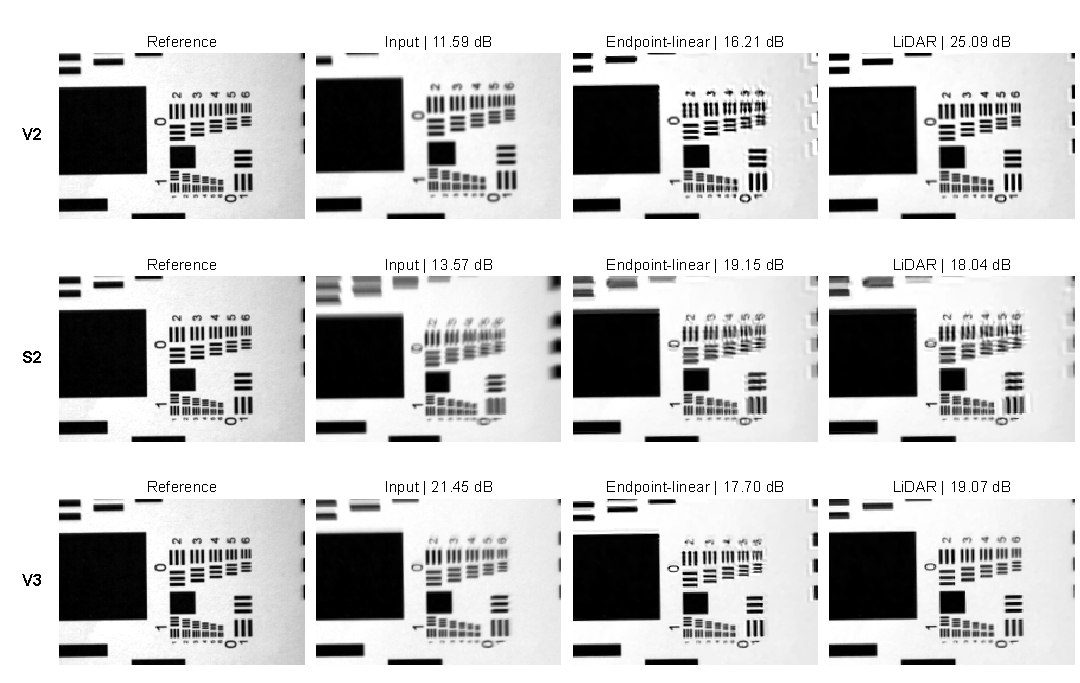
\includegraphics[width=\textwidth]{images/reconstruction_examples.pdf}
\caption{Three outcomes shown with the same canonical crop and linear grayscale range $[0,1]$. V2 has the largest measured-depth advantage; S2 favours endpoint-linear; V3 favours the input over either reconstruction. All six trials appear in Table~\ref{tab:six} and the full analysis gallery. Scoring follows the irregular common mask within each display crop.}
\label{fig:images}
\end{figure*}

\begin{table}[t]
\caption{Six independent coded exposures scored on the common canonical mask. I: blurred input; C: endpoint-linear; L: LiDAR. S/V denote smooth/variable push instructions, with independent repeats numbered 1--3. Actual velocity can vary under either instruction.}
\label{tab:six}\centering
\setlength{\tabcolsep}{3.3pt}\small
\begin{tabular}{lrrr|rrr}\hline
 & \multicolumn{3}{c|}{PSNR (dB)} & \multicolumn{3}{c}{SSIM}\\
Trial & I & C & L & I & C & L\\\hline
S1 & 15.13 & 18.08 & 18.21 & 0.646 & 0.728 & 0.767 \\
S2 & 13.57 & 19.15 & 18.04 & 0.564 & 0.789 & 0.765 \\
S3 & 16.40 & 14.33 & 18.38 & 0.712 & 0.664 & 0.777 \\
V1 & 18.71 & 14.29 & 19.22 & 0.791 & 0.647 & 0.826 \\
V2 & 11.59 & 16.21 & 25.09 & 0.523 & 0.745 & 0.906 \\
V3 & 21.45 & 17.70 & 19.07 & 0.878 & 0.803 & 0.840 \\
\hline\end{tabular}
\end{table}

Measured depth beats endpoint-linear in five of six trials on both metrics. Mean paired differences are $+3.038\pm3.666$\,dB and $+0.0843\pm0.0797$, respectively (sample SD across six independent pushes). Figure~\ref{fig:paired} shows each paired difference and the mean with one sample SD. We report these as descriptive statistics. Against the blurred input, mean gains are $+3.523\pm5.421$\,dB and $+0.1280\pm0.1485$, also with five positive trials. The median paired PSNR gain is 2.706\,dB. Leaving out each push in turn gives mean gains of 1.870--3.869\,dB; omitting V2, the largest gain, gives 1.870\,dB. The primary result retains all six trials; these omissions only check how much each push affects the mean.

\begin{figure}[t]
\centering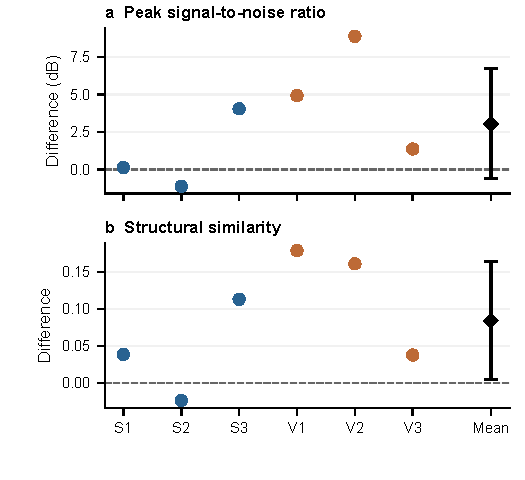
\includegraphics[width=\columnwidth]{images/paired_effects.pdf}
\caption{LiDAR-minus-endpoint-linear differences for all six coded images. The black diamond shows the mean and one sample SD; it is separate from the six trials and does not show a confidence interval. Blue: smooth instructions; orange: variable instructions.}
\label{fig:paired}
\end{figure}

S2 loses 1.115\,dB and 0.0239 SSIM to the endpoint-linear model, although both reconstructions beat its input. V3 improves over endpoint-linear but loses 2.383\,dB and 0.0380 SSIM to input. V2 has the largest paired PSNR gain, 8.880\,dB. Figure~\ref{fig:images} shows V2 and both failure types. These are two different failures: measured depth can lose to the simpler motion model, and motion inversion can degrade an already better input.



\Needspace{24\baselineskip}
\subsection{Examining the failed comparisons}
S2 stays below endpoint-linear across all 13 one-factor settings, with paired PSNR differences from $-1.209$ to $-0.847$\,dB. Changing the tested timing, TV weight, light floor, depth offset or rotation does not reverse that result. This persistence still leaves its physical cause unresolved.

For V3, denoise-only processing gives 21.43\,dB, close to the 21.45\,dB input, while LiDAR inversion gives 19.07\,dB. Most of the loss appears when the motion model is inverted. Increasing the solver from 320 to 640 iterations leaves the score at 19.07\,dB; 96 integration bins give 19.10\,dB. Tested TV weights from 0.0005 to 0.02 give 19.04--19.12\,dB. The loss persists in these checks. Equation~\eqref{eq:forward} fits the recorded blur, so errors in the assumed motion or illumination can lead the solver away from the static reference. Pose, defocus, lighting and timing remain possible contributors; these tests do not separate their effects.

\subsection{Steady-white controls and repeat variation}
Table~\ref{tab:groups} summarizes all 12 primary pushes, with only three independent repeats per cell. The variable-coded cell has a larger mean model advantage than the smooth-coded cell. White-variable reconstruction beats endpoint-linear on average but loses to the input. Motion and integrated illumination differ between the white and coded pushes, preventing a causal comparison of coding.

\begin{table}[t]
\caption{All primary cells, $n=3$ independent pushes each. $\Delta_{LC}$ is LiDAR minus endpoint-linear PSNR (mean $\pm$ sample SD); $\Delta_{LI}$ is LiDAR minus input, also as mean $\pm$ sample SD. Per-trial scores are supplied.}
\label{tab:groups}\centering\footnotesize
\begin{tabular}{llrr}\hline
Light & Instruction & $\Delta_{LC}$ (dB) & $\Delta_{LI}$ (dB)\\\hline
Coded & Smooth & $1.020\pm2.694$ & $3.174\pm1.248$\\
Coded & Variable & $5.057\pm3.758$ & $3.871\pm8.458$\\
White & Smooth & $1.549\pm2.370$ & $3.422\pm2.840$\\
White & Variable & $1.396\pm2.118$ & $-0.932\pm0.898$\\\hline
\end{tabular}
\end{table}

\subsection{Stationary and sensitivity controls}
Relative to denoise-only processing, measured-depth reconstruction gains $3.522\pm5.411$\,dB on average (sample SD, $n=6$), with five trials improving in both metrics. Thus TV denoising alone does not account for the observed mean gain.

Three static depth-driven controls change PSNR by only $+0.001$, $+0.026$ and $+0.010$\,dB relative to input, with SSIM changes $-0.0029$, $-0.0028$ and $-0.0022$. The small changes show how the pipeline behaves without target motion; they provide a control for the moving trials.

\Needspace{14\baselineskip}
Thirteen one-factor checks vary TV weight, light offset, depth timing ($\pm50$\,ms), black-state floor, common depth offset ($\pm22$\,mm) and endpoint rotation. Mean coded LiDAR advantage remains 2.43--3.56\,dB, while individual trial signs can change. This range describes the settings tested separately; it gives neither a statistical uncertainty bound nor a joint worst-case result. Doubling quadrature bins changes the mean advantage from 3.038 to 3.013\,dB. Frozen-geometry replay in a compatible numerical environment changes PSNR by at most 0.0032\,dB, showing that the frozen-geometry calculation is repeatable. Fresh registration can still change subpixel fits.
